\chapter{.NET}
\label{cha:wstep}

%https://docs.microsoft.com/en-us/dotnet/standard/tour
.NET jest platformą programistyczną umożliwiającą pisanie nowoczesnych aplikacji w językach wysokiego poziomu, do których zalicza się m.in C\# , VB oraz F\#. Platforma ta wyróżnia się tym iż:
\begin{itemize}
	\item Pozwala na użycie wielu języków programowania podczas pisania naszych programów
	\item Ma zaimplementowane mechanizmy do obsługi operacji asynchronicznych i współbieżnych
	\item Można ją stosować na różnych platformach, które posiadają środowisko wykonywalne .NET
\end{itemize}
Wszystkie języki używane w platformie .NET kompilowane są do Wspólnego Języka Pośredniego (po ang. \textit{Common Intermediate Language}), który następnie jest tłumaczony na kod bajtowy i wykonywany za pomocą środowiska wykonywalnego danej implementacji .NET.

\begin{lstlisting}[frame=single, numbers=none,captionpos=b, 
caption={Przykładowy kod aplikacji "Hello World" w języku CIL}]
.assembly HelloWorld
.class auto ansi HelloWorldApp
{
     .method public hidebysig static void Main() cil managed
     {
          .entrypoint
          .maxstack 1
          ldstr "Hello world."
          call void [mscorlib]System.Console::WriteLine(string)
          ret
     }
}
\end{lstlisting}

%https://docs.microsoft.com/en-us/dotnet/standard/tour
% CLI ECMA http://www.ecma-international.org/publications/files/ECMA-ST/ECMA-335.pdf

\section{Implementacje .NET}

Każda aplikacja .NET jest uruchamiana na jednej z implementacji .NET. \\
Od roku 2016 wprowadzono .NET Standard - wspólny zestaw API, które każda z implementacji musi posiadać. Pozwala to na pisanie i używanie bibliotek programistycznych w różnych środowiskach .NET.

Istnieją aktualnie 4 główne implementacje .NET:

%https://docs.microsoft.com/en-us/dotnet/standard/components
\subsection{.NET Core}
Został napisany z myślą o tworzeniu aplikacji cross-platformowych, które mogą zostać uruchomione na serwerach, jak i środowiskach chmurowych. Potrafi działać na platformie Windows, macOS oraz Linux. Jest to pierwsza implementacja .NET, która została zaprojektowana przez Microsoft z myślą o wieloplatformowości.

%https://docs.microsoft.com/en-us/dotnet/framework/get-started/overview
\subsection{.NET Framework}
Jest to pierwsza, oryginalna implementacja .NET, która istnieje od roku 2002. Składa się ze środowiska uruchomieniowego Common Language Runtime (CLR) oraz biblioteki standardowej zwanej jako Framework Class Library (FCL). CLR zapewnia aplikacjom wirtualną maszynę, na której wykonywany kod bajtowy skompilowany z języka CIL. Ta implementacja jest używana w tej pracy inżynierskiej.

%http://www.mono-project.com/docs/about-mono/
\subsection{Mono}
Darmowy projekt open-source prowadzony przez firmę Xamarin. Powodem stworzenia tego produktu była możliwość uruchamiania aplikacji napisanych w językach .NET na wielu platformach, jak i dostarczenie użytkownikom Linuxa narzędzi pozwalających na aplikacji w rodzinie języków .NET.
%https://docs.microsoft.com/en-us/windows/uwp/get-started/whats-a-uwp
\subsection{Universal Windows Platform (\textit{UWP})}
Implementacja, która umożliwia tworzenie aplikacji dla wszystkich platform używających Windows 10, Xboxa, niektórych urządzeń stworzonych przez Microsoft i dostosowanych urządzeń IoT.


\chapter{ASP.NET MVC}
\label{cha:wstep}
%https://msdn.microsoft.com/en-us/library/dd381412(v=vs.108).aspx

ASP.NET MVC jest frameworkiem do budowania aplikacji internetowych w oparciu o wzorzec architektoniczny Model-View-Controller (MVC). Wykorzystuje implementacje .NET Framework do uruchamiania skompilowanego kodu źródłowego.


\subsection{Model-View-Controller}

TBD

% Framework do budowania stron internetowych w oparciu o technologie .NET
\begin{figure}[h]
	\centering
	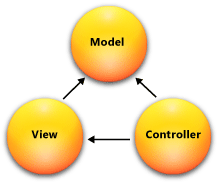
\includegraphics[height=50.5mm]{images/mvc.png}
	 \caption{Podać źródło}
\end{figure}